\hypertarget{part-1-design-1}{
\section{Part 1, design 1}\label{part-1-design-1}}

\begin{figure}[ht]
  \centering
  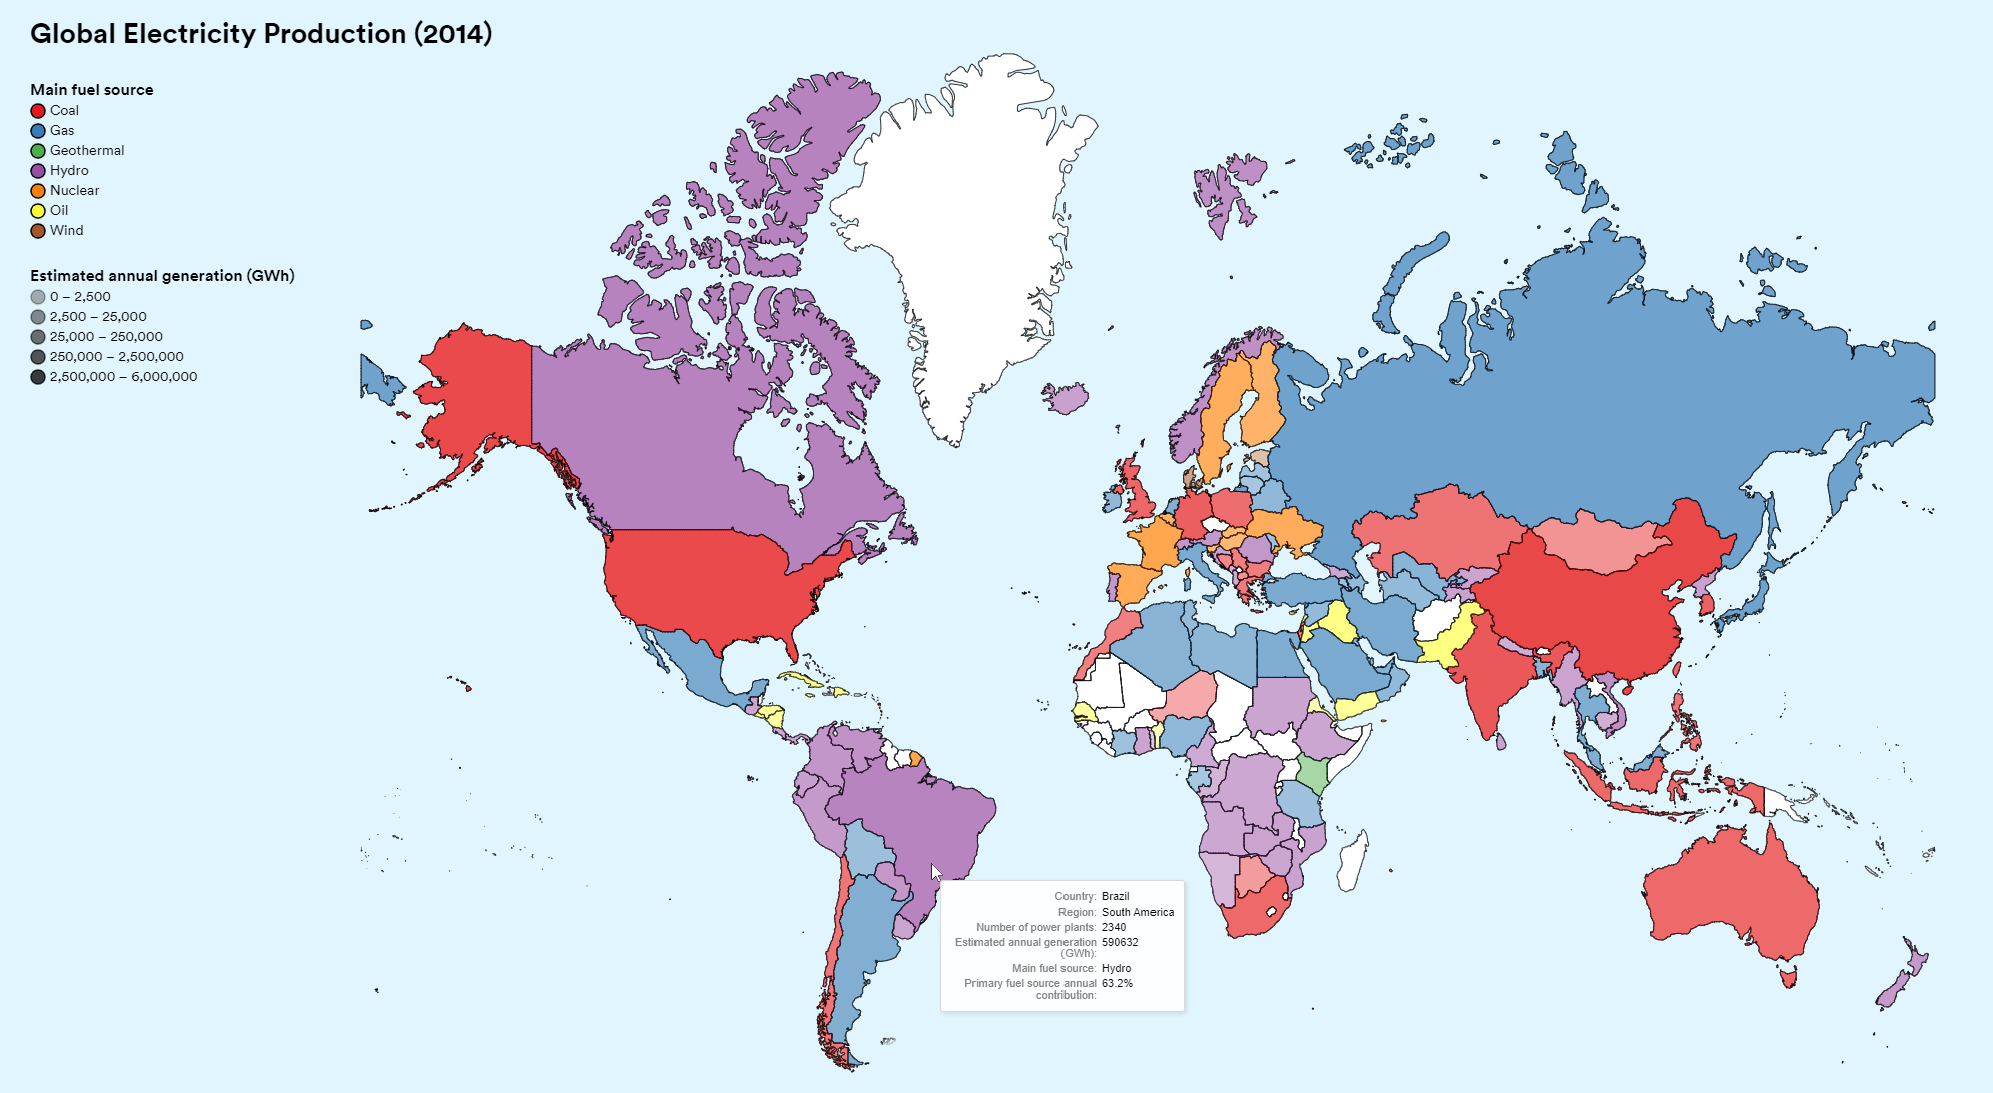
\includegraphics[width=\textwidth]{../img/design1}
  \caption{Global electricity production (Design 1)}
\end{figure}

\hypertarget{description}{
\subsubsection{Description}\label{description}}

\begin{description}
\item[Visual Design Type:]
Choropleth map
\item[Name of Tool:]
Altair
\item[Country:]
Worldwide
\item[Year:]
2014

\item[Visual Mappings:]
% each of the visual design mappings; include the data apping information about colour, shape, size, position (x/y axes), and any other visual mappings 
\begin{itemize}
  \item \textbf{Hue}: The hue of a country represents its main fuel type; the fuel type it uses to generate the most electricity.
  \item \textbf{Saturation}: The saturation of a country represents the amount of electricity it produces across all fuel types. It is banded into five discrete values along an exponential scale.
  \item \textbf{Tooltip}: Tooltips are used to offer detail-on-demand to the user, showing precise information about a country's electricity production. 
\end{itemize}

\item[Unique Observation:]
% things we can learn from the visualisation e.g. from this vis we can see this pattern
The visualisation allows the user to quickly and easily grasp the global distribution of fuel types whilst also providing a useful summary of the state of each country's power generation. For example, it is evident that coal, gas, and hydroelectric power are the major fuels across the world and that China and the United States generate the most electricity by a wide margin.

Countries' colour can be compared at a glance to get an idea of how big and varied the energy market is in a specific region. We can hover over Brasil for example, to see that hydroelectric power provides around two-thirds of the country's power - and by looking at the saturation of neighbouring countries we can see that Brasil is also the largest producer in the region of South America.

The contrasting hues also make it easy to spot countries with less common fuel types, for example we can see that Kenya is the only country in the world to favour geothermal power, and that Estonia is almost completely wind powered.

\item[Data Preparation:]
% any modifications to the original data that had to be performed to generate your beautiful image
In order to generate the map, the provided GPPD data set was combined with an open source GeoJSON map of the world so that each country's shape could be coloured. The power generation figures for each country were gathered by combining the 2014 US EPA Global Estimates (\texttt{`estimated\char`_generation\char`_gwh'}) with the 2014 national estimates (\texttt{`global\char`_generation\char`_2014'}).

Data was also aggregated through several \texttt{groupby} commands to form country-level generation and capacity figures, total number of power plants per country, and for finding out which fuel type produces the most power per country.

\end{description}

% Describe the insight that your visualizations provide. What can we learn from
% your visualizations? How are they better than a standard line, pie, or bar
% chart?